%==============================================================================
% Figure: Zero-Point Energy Density Spectrum
% Purpose: Visualize frequency-dependent ZPE density with omega^3 scaling
% Chapter: Ch08 - Aether Framework ZPE
% Type: Data/Schematic
%==============================================================================

\begin{figure}[htbp]
  \centering
  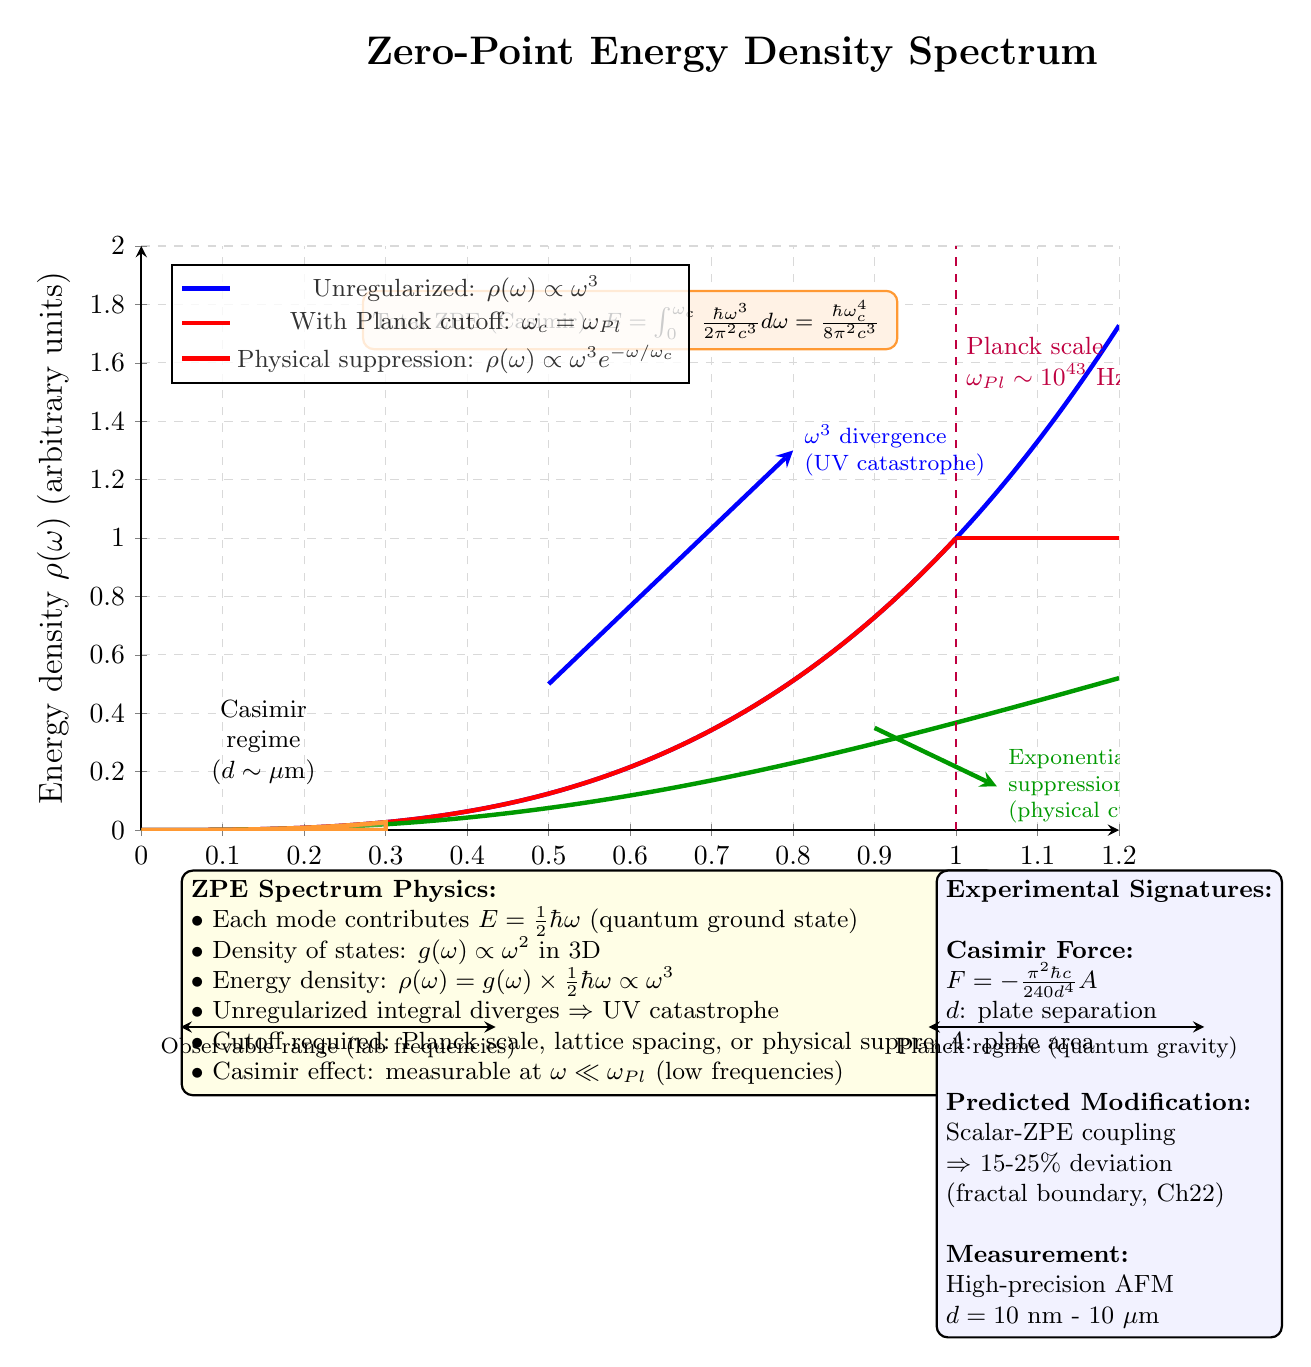
\begin{tikzpicture}[
    scale=1.0
  ]

    \begin{axis}[
      width=14cm,
      height=9cm,
      xlabel={Frequency $\omega$ (in units of $\omega_{\text{Pl}} = M_{\text{Pl}}c^2/\hbar$)},
      ylabel={Energy density $\rho(\omega)$ (arbitrary units)},
      xlabel style={font=\large},
      ylabel style={font=\large},
      xmin=0, xmax=1.2,
      ymin=0, ymax=2.0,
      axis lines=left,
      grid=major,
      grid style={dashed, gray!30},
      legend pos=north west,
      legend style={font=\small, fill=white, fill opacity=0.8},
      samples=300,
      smooth,
      thick,
      xmode=linear,
      ymode=linear
    ]

      % Unregularized ZPE: rho ~ omega^3
      \addplot[blue, ultra thick, domain=0:1.2] {x^3};
      \addlegendentry{Unregularized: $\rho(\omega) \propto \omega^3$}

      % With cutoff at Planck scale
      \addplot[red, ultra thick, domain=0:1.0] {x^3};
      \addplot[red, ultra thick, domain=1.0:1.2] {1.0};
      \addlegendentry{With Planck cutoff: $\omega_c = \omega_{\text{Pl}}$}

      % With exponential suppression (physical regularization)
      \addplot[green!60!black, ultra thick, domain=0:1.2] {x^3 * exp(-x/1.0)};
      \addlegendentry{Physical suppression: $\rho(\omega) \propto \omega^3 e^{-\omega/\omega_c}$}

      % Casimir integration region
      \addplot[orange!80, ultra thick, fill=orange!20, fill opacity=0.3, domain=0:0.3] {x^3} \closedcycle;
      \node[font=\small, align=center] at (axis cs:0.15, 0.3) {Casimir\\regime\\($d \sim \mu$m)};

      % Vertical line at cutoff
      \draw[dashed, thick, purple] (axis cs:1.0, 0) -- (axis cs:1.0, 2.0)
        node[pos=0.8, right, font=\small, align=left] {Planck scale\\$\omega_{\text{Pl}} \sim 10^{43}$ Hz};

      % Annotation arrows
      \draw[->, >=stealth, ultra thick, blue] (axis cs:0.5, 0.5) -- (axis cs:0.8, 1.3)
        node[right, align=left, font=\footnotesize] {$\omega^3$ divergence\\(UV catastrophe)};

      \draw[->, >=stealth, ultra thick, green!60!black] (axis cs:0.9, 0.35) -- (axis cs:1.05, 0.15)
        node[right, align=left, font=\footnotesize] {Exponential\\suppression\\(physical cutoff)};

      % Integration formula annotation
      \node[anchor=north, align=center, font=\footnotesize, draw=orange!80, fill=orange!10, rounded corners]
        at (axis cs:0.6, 1.85) {
        Total ZPE (Casimir): $E = \int_0^{\omega_c} \frac{\hbar\omega^3}{2\pi^2 c^3} d\omega = \frac{\hbar\omega_c^4}{8\pi^2 c^3}$
      };

    \end{axis}

    % Physics explanation box
    \node[anchor=north west, align=left, font=\small, draw=black, fill=yellow!10, rounded corners, thick]
      at (0.5, -0.5) {
      \textbf{ZPE Spectrum Physics:} \\
      $\bullet$ Each mode contributes $E = \frac{1}{2}\hbar\omega$ (quantum ground state) \\
      $\bullet$ Density of states: $g(\omega) \propto \omega^2$ in 3D \\
      $\bullet$ Energy density: $\rho(\omega) = g(\omega) \times \frac{1}{2}\hbar\omega \propto \omega^3$ \\
      $\bullet$ Unregularized integral diverges $\Rightarrow$ UV catastrophe \\
      $\bullet$ Cutoff required: Planck scale, lattice spacing, or physical suppression \\
      $\bullet$ Casimir effect: measurable at $\omega \ll \omega_{\text{Pl}}$ (low frequencies)
    };

    % Experimental connection box
    \node[anchor=north east, align=left, font=\small, draw=black, fill=blue!5, rounded corners, thick]
      at (14.5, -0.5) {
      \textbf{Experimental Signatures:} \\
      \\
      \textbf{Casimir Force:} \\
      $F = -\frac{\pi^2\hbar c}{240 d^4} A$ \\
      $d$: plate separation \\
      $A$: plate area \\
      \\
      \textbf{Predicted Modification:} \\
      Scalar-ZPE coupling \\
      $\Rightarrow$ 15-25\% deviation \\
      (fractal boundary, Ch22) \\
      \\
      \textbf{Measurement:} \\
      High-precision AFM \\
      $d = 10$ nm - 10 $\mu$m
    };

    % Title
    \node[anchor=south, font=\Large\bfseries] at (7.5, 9.5) {Zero-Point Energy Density Spectrum};

    % Scale markers
    \draw[<->, >=stealth, thick] (0.5, -2.5) -- (4.5, -2.5)
      node[midway, below, font=\footnotesize] {Observable range (lab frequencies)};
    \draw[<->, >=stealth, thick] (10.0, -2.5) -- (13.5, -2.5)
      node[midway, below, font=\footnotesize] {Planck regime (quantum gravity)};

  \end{tikzpicture}
  \caption{Zero-point energy (ZPE) density spectrum as a function of frequency $\omega$. The
    unregularized spectrum (blue) follows $\rho(\omega) \propto \omega^3$, arising from the
    product of the 3D density of states ($g(\omega) \propto \omega^2$) and the quantum ground-state
    energy ($\frac{1}{2}\hbar\omega$). This leads to ultraviolet divergence if integrated to
    infinite frequency. A hard cutoff at the Planck scale (red) truncates the divergence, while
    physical regularization mechanisms (green) provide exponential suppression. The orange shaded
    region shows the integration domain for Casimir effect calculations at laboratory scales
    ($d \sim \mu$m, $\omega_c \sim c/d$). The Aether framework predicts modifications to the
    Casimir force (15-25\% deviations) via scalar field coupling to ZPE, testable in precision
    experiments with fractal boundary geometries (Ch22 protocols).}
  \label{fig:zpe-density-spectrum}
\end{figure}
